\documentclass[b5paper, twoside, 9pt]{book}
% \documentclass[a4paper, twoside, 9pt]{book}

\usepackage{sectsty}
\allsectionsfont{\usefont{T1}{phv}{bc}{n}\selectfont}
\usepackage[Lenny]{../fncychapleo}
\usepackage{makeidx}
\usepackage{graphicx}
\usepackage[absolute]{textpos} % PDF Cover
\usepackage{multicol}
\usepackage{float}
\usepackage{listings}
\usepackage{color}
\usepackage{textcomp}
\usepackage{alltt}
\usepackage{times}
\usepackage{ifpdf}

\ifpdf
\usepackage[pdftex,
			pagebackref=false,
            colorlinks=true,
            linkcolor=black,
			citecolor=black,
			anchorcolor=black,
			filecolor=black,
			menucolor=black,
			urlcolor=black,
			pdftitle={Fuzzy Logic Tools Reference Manual v1.0},
			pdfsubject={University of Huelva, Spain, 2011},
			pdfauthor={Antonio Javier Barragan Pi\~na \& Jos\'e Manuel And\'ujar M\'arquez},
			pdfkeywords={This work is licensed under a Creative Commons Attribution-ShareAlike 3.0 License.},
            unicode
           ]{hyperref}
\else
\usepackage[ps2pdf,
			pagebackref=false,
            colorlinks=true,
            linkcolor=black,
			citecolor=black,
			anchorcolor=black,
			filecolor=black,
			menucolor=black,
			urlcolor=black,
			pdftitle={Fuzzy Logic Tools Reference Manual v1.0},
			pdfsubject={University of Huelva, Spain, 2011},
			pdfauthor={Antonio Javier Barragan Pi\~na \& Jos\'e Manuel And\'ujar M\'arquez},
			pdfkeywords={This work is licensed under a Creative Commons Attribution-ShareAlike 3.0 License.},
            unicode
           ]{hyperref}
\usepackage{pspicture}
\fi

\usepackage[nottoc]{tocbibind}
\usepackage[utf8]{inputenc}
\usepackage{amstext}
\usepackage{../doxygen_changed}
\lstset{language=C++,inputencoding=utf8,basicstyle=\footnotesize,
        breaklines=true,breakatwhitespace=true,tabsize=8,numbers=left}
\makeindex
\setcounter{tocdepth}{3}
\renewcommand{\footrulewidth}{0.4pt}

\renewcommand{\tt}{}

\clubpenalty=1000
\widowpenalty=10000

\usepackage[hmarginratio=1:1]{geometry} % ########## To create the PDF in A4 format with crop marks ##########
% \usepackage[cam,a4,center,odd]{crop}    % ##########                Place crop marks                ##########

\begin{document}
\hypersetup{pageanchor=false}

{\thispagestyle{empty}
% \begin{textblock*}{297mm}(-17mm,-24mm) % A4
% 	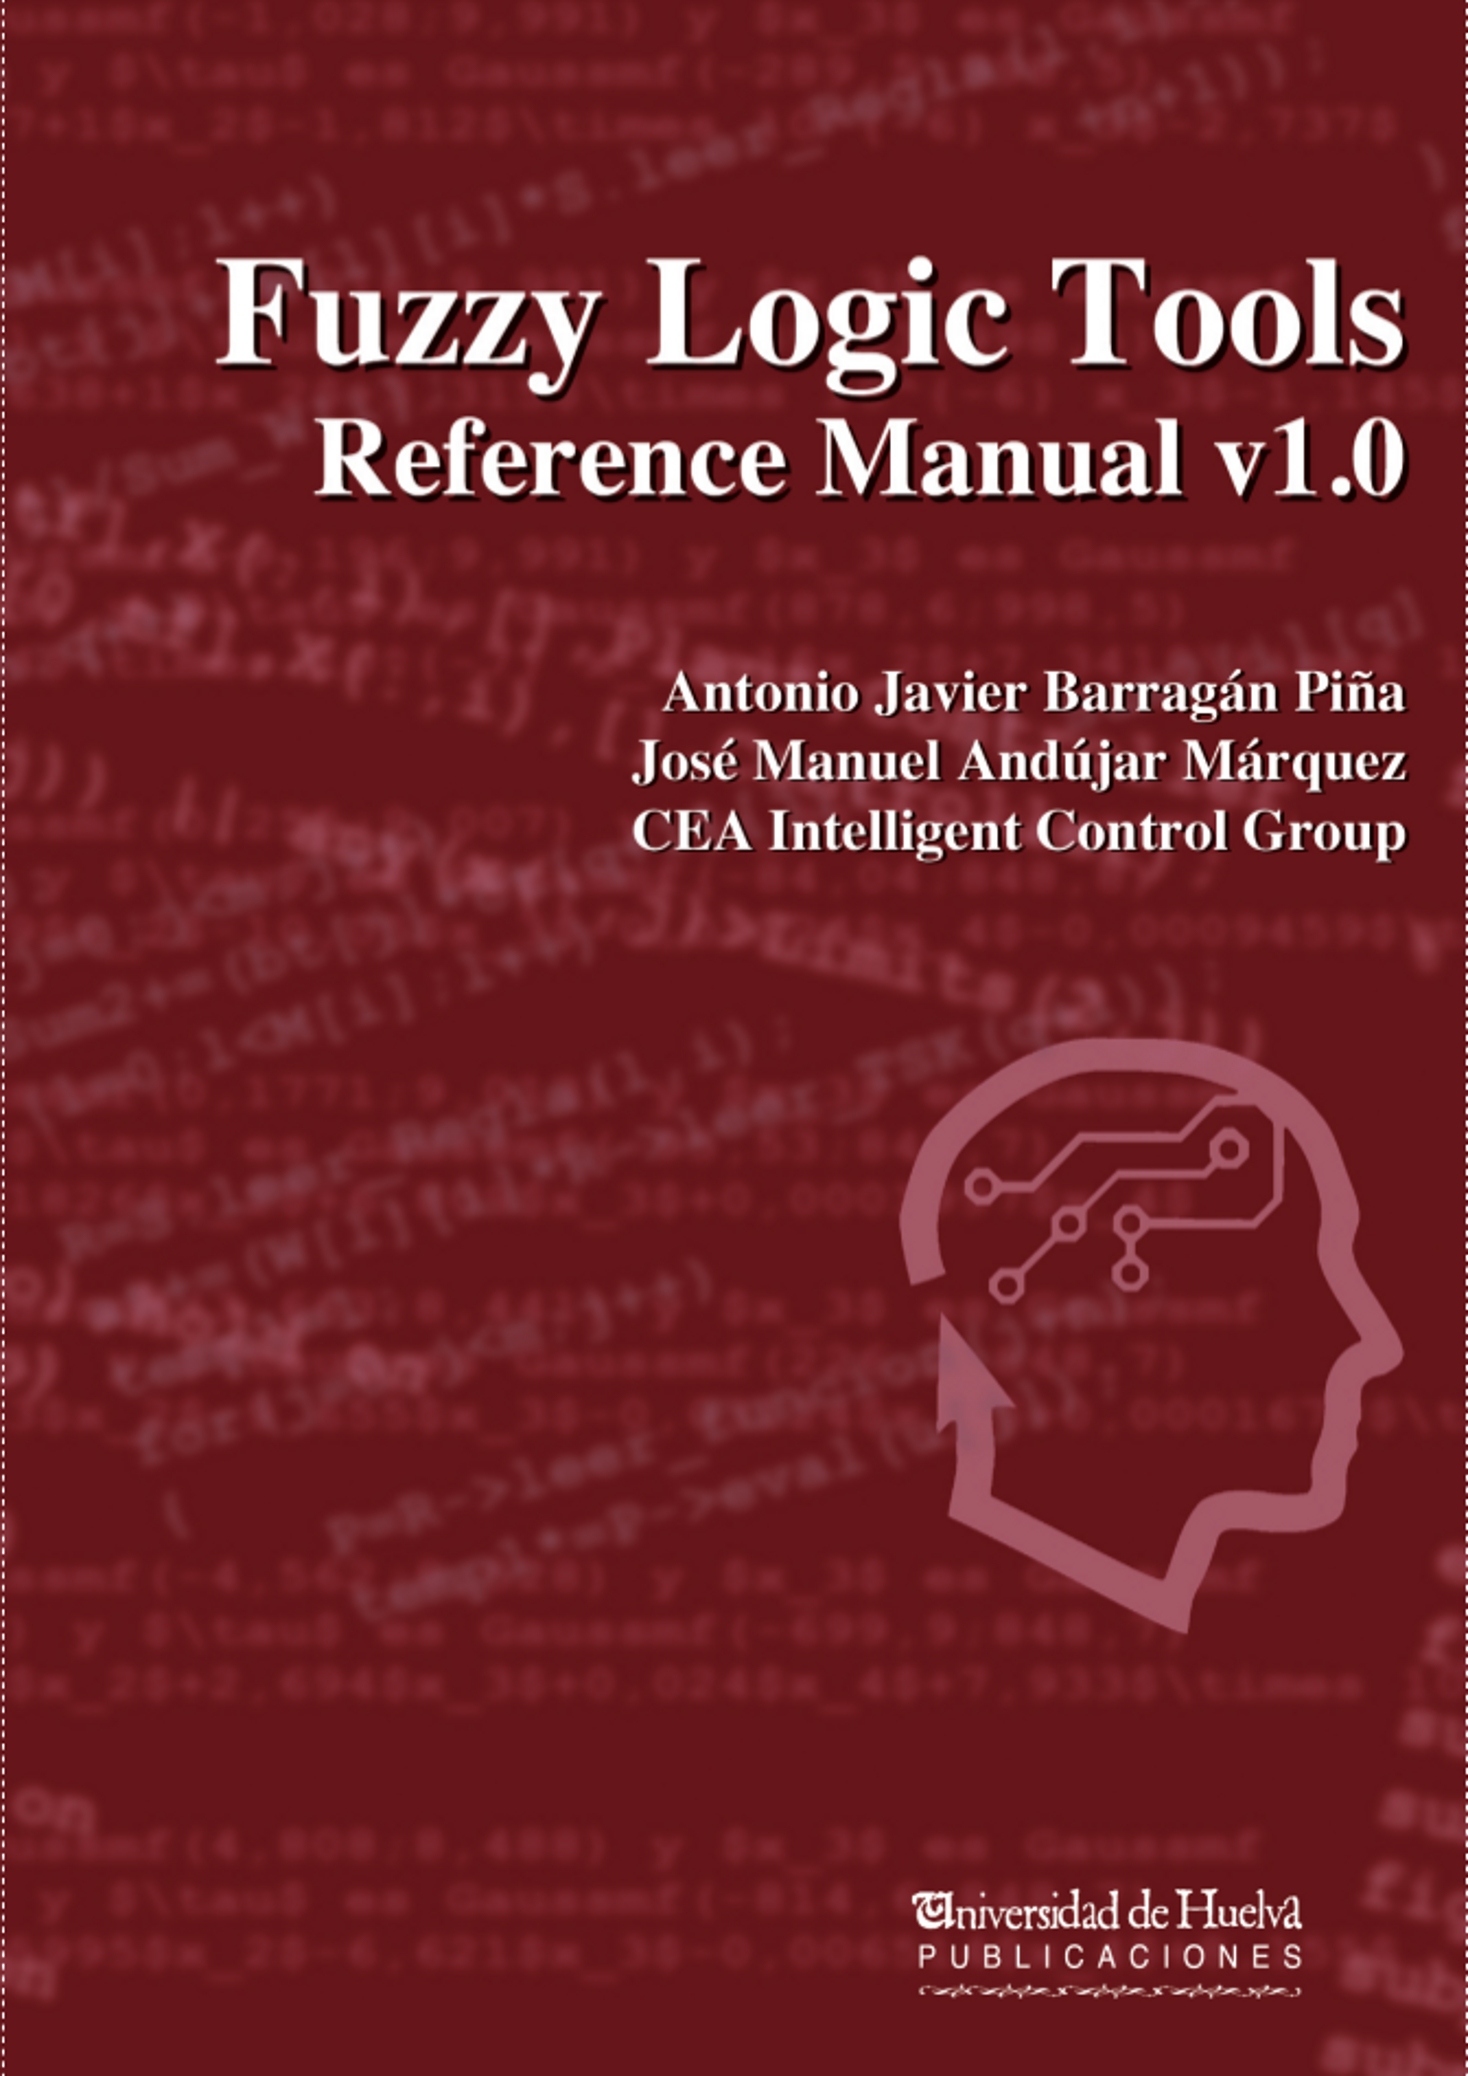
\includegraphics[height=298mm,width=210mm]{../front}
% \end{textblock*}

\begin{textblock*}{250mm}(0mm,0mm) % B5
	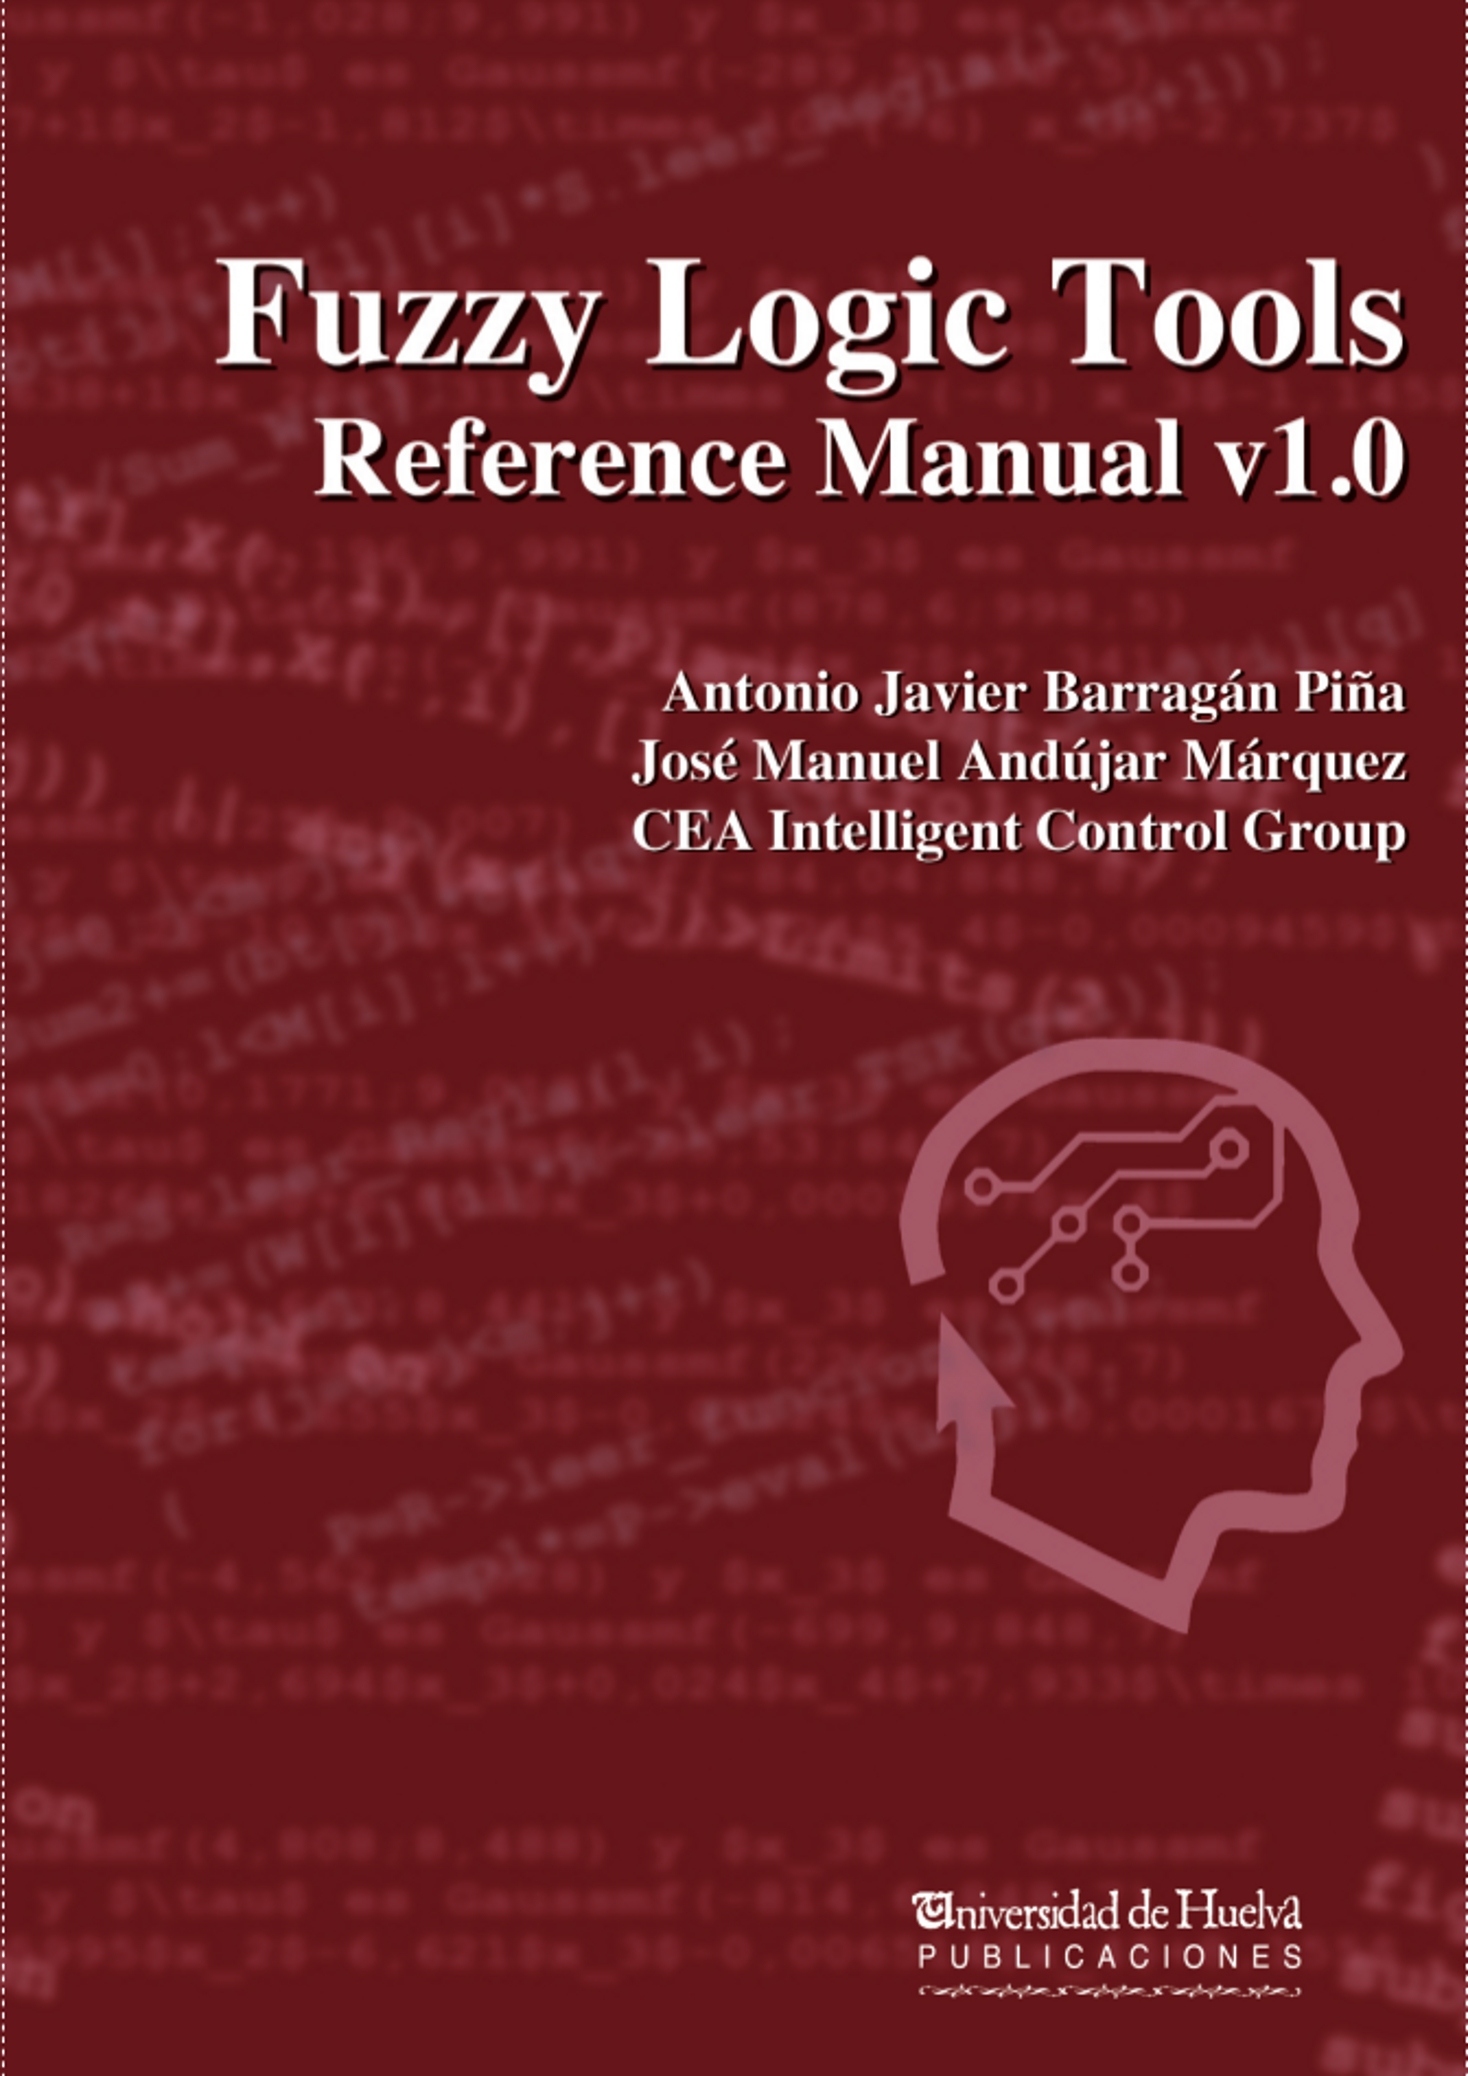
\includegraphics[height=250mm,width=176mm]{../front}
\end{textblock*}
}
~\newpage\cleardoublepage
% -----------------------------------------------------------------------------------------------------------

\begin{titlepage}
\begin{center}
{\LARGE Fuzzy Logic Tools Reference Manual\\[1ex]\Large v1.0}\\
\vspace*{2cm}
{\Large Antonio Javier Barragán Piña\\
\vspace{5mm}
José Manuel Andújar Márquez}\\
\vspace*{6cm}
{\Large University of Huelva, Spain\\May 2011}\\
\vspace*{1cm}
{
\includegraphics[width=30mm]{../logouhu}}
\end{center}
\end{titlepage}
\clearpage\newpage

{\thispagestyle{empty}
\begin{center}
FUZZY LOGIC TOOLS REFERENCE MANUAL v1.0
\\\vspace{0.5cm}
\textcopyright 2011 Antonio Javier Barragan Pi\~na \& Jos\'e Manuel And\'ujar M\'arquez

Publication Service of the University of Huelva

Further information about this book is available at \url{http://uhu.es/antonio.barragan/flt}
\end{center}

{\footnotesize\vfill
\textbf{Permission is granted to copy, distribute and/or modify this document
under the terms of the Creative Commons Attribution 3.0 License}.
You are free to share, copy, distribute, transmit, remix and adapt this work,
but you must attribute the work in the manner specified by the author or licensor
(but not in any way that suggests that they endorse you or your use of the work).

With the understanding that:
\begin{itemize}
  \item Waiver: Any of the above conditions can be waived if you get permission from
	the copyright holder.
  \item Public Domain: Where the work or any of its elements is in the public domain
	under applicable law, that status is in no way affected by the license.
  \item Other Rights: In no way are any of the following rights affected by the
	license:
  \begin{itemize}
	\item Your fair dealing or fair use rights, or other applicable copyright
	  exceptions and limitations.
	\item The author's moral rights.
	\item Rights other persons may have either in the work itself or in how the work is
	  used, such as publicity or privacy rights.
  \end{itemize}
  \item Notice: For any reuse or distribution, you must make clear to others the license
	terms of this work.
\end{itemize}

To view a copy of the full license, please go to \url{http://creativecommons.org/licenses/by/3.0/}
or send a letter to Creative Commons, 171 Second Street, Suite 300, San Francisco,
California 94105, USA.

This book has been generated by Doxygen
(\url{http://www.stack.nl/~dimitri/doxygen}) and it has subsequently been
revised and edited by the authors.

\textbf{Fuzzy Logic Tools (FLT) is licensed under the GNU/GPLv3 or
higher\footnote{The GNU General Public License is a free, copyleft license for
software and other kinds of works.}}. You can view this license at: \url{http://www.gnu.org/licenses/gpl.html}

FLT has been written in C++. This software has been compiled and tested in 32 and
64 bits architectures on GNU/Linux
using GCC (\url{http://gcc.gnu.org}), and in 32 bits architectures on Microsoft
\mbox{Windows\textsuperscript{\tiny\textregistered}} operating
systems\footnote{The Microsoft brand name and is owned by Microsoft Corporation
(\url{http://www.microsoft.com}).} using MinGW (\url{http://www.mingw.org}).

This text provides some useful functions for use with
\mbox{MATLAB\textsuperscript{\tiny\textregistered}} API\footnote{Currently the
license of \mbox{MATLAB\textsuperscript{\tiny\textregistered}} is owned by
MathWorks MATLAB Inc.}. The authors recommend that you use GNUMex
(\url{http://gnumex.sourceforge.net}) to compile MEX files in Microsoft
\mbox{Windows\textsuperscript{\tiny\textregistered}} operating systems.

\textbf{ISBN}: 978-84-15147-32-9.

\textbf{Legal Deposit}: H 125-2012.
}

% Prueba de referencias: \cite{Andujar2010, Andujar2005b, Andujar2009, JavierBarraganTesis, Barragan2011, Barragan2011a, Jimenez2008}
~\newpage\cleardoublepage
\pagenumbering{roman}

%% Page headers
  \frontmatter{}
  \fancyhead[RO]{{\footnotesize\rightmark}\hspace{2em}\thepage}
  \setcounter{tocdepth}{2}
  \fancyhead[LE]{\thepage\hspace{2em}\footnotesize{\leftmark}}
  \fancyhead[RE,LO]{}
  \fancyhead[RO]{{\footnotesize\rightmark}\hspace{2em}\thepage}
%   \setlength\headheight{14.5pt}

\chapter*{Preface} % --------------------------------------------------------------------
This manual documents the use of Fuzzy Logic Tools (FLT), a C++ framework for storage,
analysis and design of fully general multiple-input multiple-output (MIMO) Takagi-Sugeno
fuzzy control systems, without constraints in the order of either the inputs or the output
vectors.

This reference manual is intended as a reference work for those developers wishing to use the tools provided by the FLT. Therefore, the text is structured following the typical pattern of reference manuals. Firstly, a general description of the variables, functions, classes, methods and attributes included in the software is presented. Then each of these items is studied in depth. Finally, some examples of using the FLT are included. These functions can be used for the analysis and design of TS-type fuzzy control.

With the intention of making our work available to the entire scientific community, FLT is licensed under GPLv3, so you can use it freely if it meets the requirements of such license (see http://www.gnu.org/licenses/gpl.html). With the same intention, this document is licensed under a Creative Commons Attribution-ShareAlike 3.0 License, approved for Free Cultural Works initiative.

This work is in continuous evolution and improvement. If you are interested can stay informed of new versions, bugs, and other information about the project at \url{http://uhu.es/antonio.barragan/flt}

\begin{flushright}
Jos\'e Manuel And\'ujar M\'arquez\\
May 2011
\end{flushright}

% ---------------------------------------------------------------------------------------

\clearemptydoublepage
\tableofcontents
\clearemptydoublepage

\pagenumbering{arabic}
\hypersetup{pageanchor=true}

%% Principal pages headers
	\mainmatter{}\fancyhead[RE,LO]{\thesection}

% ########### From here, the code is generated by Doxygen ###########
%
% Changes to do from here to obtain the structure of "Fuzzy Logic Tools Reference Manual"
%
% Comment all \chapter{XXXX Index} from the beginning to "Namespace Documentation" (do not comment the \input{.} command!
%
% Reorder the "Class Documentation" chapter:
%	1st Membership, then all membership functions:
% 	  (anymf, ..., zmf // [gaussmf before gauss2mf, sigmf before sig2mf and psigmf]), and finally, rule and system clases.
%
% Reorder the "File Documentation" chapter:
%	1st messages, then membership, rule, system, utilities, fuzzyIO, derivatives, Kalman, and finally, aux_matlab and tnt_extensions.
%
% Important: Some images must be edited manually to avoid exceeding the margins:
% In Membersip class:
% 	\begin{figure}
% 	Inheritance diagram for FLT::Membership:
% 	\begin{center}
% 	\leavevmode
% 	\includegraphics[width=215pt]{df/df2/class_f_l_t_1_1_membership__inherit__graph}
% 	\end{center}
% 	\end{figure}
%
% In Membersip file:
% \resizebox{\linewidth}{!}{\includegraphics[width=400pt]{d5/d09/membership_8hpp__incl}}
%
% In Rule file:
% 	\includegraphics[width=341pt]{d2/d52/rule_8hpp__incl}
% 	\end{center}
% 	\end{figure}
% 	This graph shows which files directly or indirectly include this file:\nopagebreak
% 	\begin{figure}[H]
% 	\begin{center}
% 	\leavevmode
% 	\includegraphics[width=309pt]{d2/d9f/rule_8hpp__dep__incl}
% 	\end{center}
% 	\end{figure}\clearpage
%
% In System file:
% \resizebox{\linewidth}{!}{\includegraphics[width=400pt]{d4/db3/system_8hpp__incl}}
% 	\end{center}
% 	\end{figure}\clearpage
%
% In Utilities file:
% \resizebox{\linewidth}{!}{\includegraphics[width=400pt]{df/d46/utilities_8hpp__incl}}
% 	\end{center}
% 	\end{figure}\clearpage
%
% In fuzzy_IO file:
% \resizebox{\linewidth}{!}{\includegraphics[width=400pt]{d5/d0a/fuzzy_i_o_8hpp__incl}}
%
% In Derivatives file:
% \resizebox{\linewidth}{!}{\includegraphics[width=400pt]{d7/d54/derivatives_8hpp__incl}}
% 	\end{center}
% 	\end{figure}\clearpage
%
% In Kalman file:
% \resizebox{\linewidth}{!}{\includegraphics[width=400pt]{d0/d7a/_kalman_8hpp__incl}}
%
% In aux_mat file:
% \resizebox{\linewidth}{!}{\includegraphics[width=400pt]{dd/d70/aux__matlab_8hpp__incl}}
%
%
% If necessary, include these lines at the end of the document, before "\end{document}":
% 	  \bibliographystyle{apalike}
% 	  \bibliography{../references}
%
% \chapter{Fuzzy Logic Tools}
% \label{index}\hypertarget{index}{}\input{index}
% % \chapter{Namespace Index}
% \input{namespaces}
% % \chapter{Class Index}
% \input{hierarchy}
% % \chapter{Class Index}
% \input{annotated}
% % \chapter{File Index}
% \input{files}
% \chapter{Namespace Documentation}
% \input{db/de5/namespace_f_l_t}
% \chapter{Class Documentation}
% \input{d0/d45/class_f_l_t_1_1_membership}
% \input{dc/d02/class_f_l_t_1_1_anymf}
% \input{da/d6c/class_f_l_t_1_1_constmf}
% \input{d1/dda/class_f_l_t_1_1_gaussmf}
% \input{d3/d2b/class_f_l_t_1_1_gauss2mf}
% \input{de/dba/class_f_l_t_1_1_g_bellmf}
% \input{d2/dc8/class_f_l_t_1_1_pimf}
% \input{d7/d76/class_f_l_t_1_1_sigmf}
% \input{d5/d29/class_f_l_t_1_1_sig2mf}
% \input{db/de3/class_f_l_t_1_1_p_sigmf}
% \input{d3/d5e/class_f_l_t_1_1_smf}
% \input{d4/d35/class_f_l_t_1_1_trapmf}
% \input{d8/d76/class_f_l_t_1_1_trimf}
% \input{dc/d0d/class_f_l_t_1_1_zmf}
% \input{da/d53/class_f_l_t_1_1_rule}
% \input{d9/d9e/class_f_l_t_1_1_system}
% \chapter{File Documentation}
% \input{d5/d48/messages_8h}
% \input{da/d12/membership_8hpp}
% \input{d3/d5f/rule_8hpp}
% \input{dd/d90/system_8hpp}
% \input{dc/d5f/utilities_8hpp}
% \input{d3/dde/fuzzy_i_o_8hpp}
% \input{d0/d98/derivatives_8hpp}
% \input{de/d17/_kalman_8hpp}
% \input{dd/d5b/aux__matlab_8hpp}
% \input{d5/d4d/tnt__extension_8hpp}
%
% % Add at the end, befor \end{document}, for the back cover
% {\thispagestyle{empty}
% \begin{textblock*}{297mm}(-18mm,-24mm) % A4
% 	
\includegraphics[height=298mm,width=211mm]{../back}
% % \end{textblock*}
%
% \begin{textblock*}{250mm}(-1mm,0mm) % B5
% 	
\includegraphics[height=250mm,width=177mm]{../back}
% \end{textblock*}
% }
%
